%% IAENG_pub.tex 2010/08/30
%% It is based on the bare_jrnl.tex V1.3 2007/01/11 by Michael Shell
%% see http://www.michaelshell.org/
%% for current contact information.
%%
%% This is a skeleton file demonstrating the use of IAENGtran.cls
%% (requires IAENGtran.cls version 1.7 or later) with an IAENG journal/conference paper.
%%
%% Support sites:
%% http://www.michaelshell.org/tex
%% http://www.ctan.org/tex-archive/macros/latex/contrib/IEEEtran/

% *** Authors should verify (and, if needed, correct) their LaTeX system  ***
% *** with the testflow diagnostic prior to trusting their LaTeX platform ***
% *** with production work. IAENG's font choices can trigger bugs that do  ***
% *** not appear when using other class files.                            ***
% The testflow support page is at:
% http://www.michaelshell.org/tex/testflow/


%%*************************************************************************
%% Legal Notice:
%% This code is offered as-is without any warranty either expressed or
%% implied; without even the implied warranty of MERCHANTABILITY or
%% FITNESS FOR A PARTICULAR PURPOSE!
%% User assumes all risk.
%% In no event shall IAENG or any contributor to this code be liable for
%% any damages or losses, including, but not limited to, incidental,
%% consequential, or any other damages, resulting from the use or misuse
%% of any information contained here.
%%
%% All comments are the opinions of their respective authors and are not
%% necessarily endorsed by the IAENG.
%%
%% This work is distributed under the LaTeX Project Public License (LPPL)
%% ( http://www.latex-project.org/ ) version 1.3, and may be freely used,
%% distributed and modified. A copy of the LPPL, version 1.3, is included
%% in the base LaTeX documentation of all distributions of LaTeX released
%% 2003/12/01 or later.
%% Retain all contribution notices and credits.
%% ** Modified files should be clearly indicated as such, including  **
%% ** renaming them and changing author support contact information. **
%%
%%*************************************************************************

% Note that the a4paper option is mainly intended so that authors in
% countries using A4 can easily print to A4 and see how their papers will
% look in print - the typesetting of the document will not typically be
% affected with changes in paper size (but the bottom and side margins will).
% Use the testflow package mentioned above to verify correct handling of
% both paper sizes by the user's LaTeX system.
%
% Also note that the "draftcls" or "draftclsnofoot", not "draft", option
% should be used if it is desired that the figures are to be displayed in
% draft mode.
%
\documentclass[journal]{IAENGtran}
%
% If IAENGtran.cls has not been installed into the LaTeX system files,
% manually specify the path to it like:
% \documentclass[journal]{../sty/IAENGtran}

% Load configuration
\usepackage{setspace}
\doublespacing

\newcommand{\ThesisProposalTH}{โครงร่างวิทยานิพนธ์}
\newcommand{\ThesisProposalEN}{Thesis Proposal}
\newcommand{\ThesisTopic}{หัวข้อวิทยานิพนธ์}

% - - - - - - - - - - - - - - - - - - - -
% Control words
% - - - - - - - - - - - - - - - - - - - -
\newcommand{\scg}{กราฟการเรียกเชิงสถิต}
\newcommand{\scgEN}{Static call graph}

\newcommand{\cfg}{กราฟการไหลของการควบคุม}
\newcommand{\cfgen}{Control flow graph}

\newcommand{\DDPath}{DD-Path}
\newcommand{\DDPathEN}{Decision-to-decision Path}

\newcommand{\FeasiblePath}{เส้นทางที่เป็นไปได้}
\newcommand{\FeasiblePathEN}{Feasible path}

\newcommand{\InfeasiblePath}{เส้นทางที่เป็นไปไม่ได้}
\newcommand{\InfeasiblePathEN}{Infeasible path}

\newcommand{\FeasibleAndInfeasiblePath}{เส้นทางที่เป็นไปได้และไม่ได้}
\newcommand{\FeasibleAndInfeasiblePathEN}{Feasib/Users/sitdh/Desktop/vector-Overwatch-Ana-wallpaper.jpg Infeasible path}

\newcommand{\sourcecode}{รหัสต้นฉบับ}

\newcommand{\TestDataGeneration}{การสร้างข้อมูลทดสอบ}
\newcommand{\TestDataGenerationEN}{Test data generation}

\newcommand{\RegressionTesting}{การทดสอบเชิงทดถอย}
\newcommand{\RegressionTestingEN}{Regression testing}

\newcommand{\Repository}{คลังข้อมูล}
\newcommand{\RepositoryEN}{Repository}

\newcommand{\softwareComponent}{ส่วนประกอบซอฟต์แวร์}
\newcommand{\softwareComponentEN}{Software component}

\newcommand{\IntegrationTesting}{การทดสอบผสาน}
\newcommand{\IntegrationTestingEN}{Integration testing}

\newcommand{\class}{คลาส}
\newcommand{\classEN}{Class}

\newcommand{\method}{\mbox{เมท็อด}}
\newcommand{\methodEN}{Method}

\newcommand{\attribute}{แอททริบิวต์}
\newcommand{\attributeEN}{Attribute}

\newcommand{\MethodSignature}{ลายเซ็นของเมธอด}
\newcommand{\MethodSignatureEN}{Method signature}

\newcommand{\DirectedMultiGraph}{กราฟหลายทางมีทิศทาง}
\newcommand{\DirectedMultiGraphEN}{Directed multigraph}

\newcommand{\DirectedGraph}{กราฟมีทิศทาง}
\newcommand{\DirectedGraphEN}{Directed graph}

\newcommand{\ProgramGraph}{กราฟโปรแกรม}
\newcommand{\ProgramGraphEN}{Program graph}

\newcommand{\BasisPath}{เส้นทางมูลฐาน}
\newcommand{\BasisPathEN}{ฺBasis paths}

\newcommand{\Node}{โหนด}
\newcommand{\NodeEN}{Node}

\newcommand{\Edge}{เส้นเชื่อม}
\newcommand{\EdgeEN}{Edge}

\newcommand{\PredicateNode}{{\Node}เงื่อนไขการดำเนินงาน}
\newcommand{\PredicateNodeEN}{Predicate node}

\newcommand{\TestPath}{เส้นทางทดสอบ}
\newcommand{\TestPathEN}{Test path}

\newcommand{\sourcenode}{โหนดต้นทาง}
\newcommand{\sourcenodeEN}{Source node}

\newcommand{\sinknode}{โหนดปลายทาง}
\newcommand{\sinknodeEN}{Sink node}

\newcommand{\Cyclomatic}{ความซับซ้อนไซโคลเมทิก}
\newcommand{\CyclomaticEN}{Cyclomatic Complexity}

\newcommand{\inputVector}{เวกเตอร์นำเข้า}
\newcommand{\inputVectorEN}{Input vector}

\newcommand{\CUT}{{\class}ภายใต้การทดสอบ}
\newcommand{\CUTEN}{Class under test}

\newcommand{\SUT}{ซอฟต์แวร์ภายใต้การทดสอบ}
\newcommand{\SUTEN}{Software under test}

\newcommand{\Path}{ทางเดิน}
\newcommand{\PathEN}{Path}

\newcommand{\DynamicInformation}{ข้อมูลเชิงพลวัต}
\newcommand{\DynamicInformationEN}{Dynamic information}

\newcommand{\StaticInformation}{ข้อมูลเชิงสถิต}
\newcommand{\StaticInformationEN}{Static information}

\newcommand{\testSuite}{ชุดทดสอบ}
\newcommand{\testSuiteEN}{Test suite}

\newcommand{\testCase}{กรณีทดสอบ}
\newcommand{\testCaseEN}{Test case}

\newcommand{\Package}{โปรแกรมสำเร็จ} % http://www.rirs3.royin.go.th
\newcommand{\PackageEN}{Package}

\newcommand{\expectedOutput}{ผลลัพธ์ที่คาดหวัง}
\newcommand{\expectedOutputEN}{Expected output}

\newcommand{\csp}{ปัญหาการหาค่าเหมาะที่สุดเชิงการจัด} % https://www.cp.eng.chula.ac.th/~somchai/CD/2110427/2546/demo/HW2-TSP/saTSP.htm
\newcommand{\cspEN}{Constraint satisfaction problem}

\newcommand{\Algorithm}{ขั้นตอนวิธี}
\newcommand{\AlgorithmEN}{Algorithm}

\newcommand{\software}{ซอฟต์แวร์}
\newcommand{\softwareEN}{Software}

\newcommand{\tester}{นักทดสอบซอฟต์แวร์}
\newcommand{\testerEN}{Software tester}

\newcommand{\constantExtracting}{การรวบรวมค่าคงที่}
\newcommand{\constantExtractingEN}{Constant extracting}

\newcommand{\graphCreation}{การสร้างกราฟ}
\newcommand{\graphCreationEN}{Graph creation}

\newcommand{\sourcecodeInstrumention}{แทรกคำสั่งในรหัสต้นฉบับ}
\newcommand{\sourcecodeInstrumentionEN}{Source code instrumentation}

\newcommand{\testcaseGeneration}{การสร้างกรณีทดสอบ}
\newcommand{\testcaseGenerationEN}{Test case generation}

\newcommand{\testpathSelection}{การเลือกทางเดินทดสอบ}
\newcommand{\testpathSelectionEN}{Test path selection}

\newcommand{\randomTestData}{สุ่มข้อมูลนำเข้า}
\newcommand{\randomTestDataEN}{Random test data}

\newcommand{\testData}{ข้อมูลทดสอบ}
\newcommand{\testDataEN}{Test data}

\newcommand{\testCaseGeneration}{การสร้างกรณีทดสอบ}
\newcommand{\testCaseGenerationEN}{Test case generation}

\newcommand{\expectedOutputAdjustment}{การปรับค่าคาดหวัง}
\newcommand{\expectedOutputAdjustmentEN}{Expected output adjustment}

\newcommand{\executeSoftwareTesting}{ดำเนินการทดสอบซอฟต์แวร์}
\newcommand{\executeSoftwareTestingEN}{Software testing execute}

\newcommand{\testResultCompare}{เปรียบเทียบผลลัพธ์การดำเนินงาน}
\newcommand{\testResultCompareEN}{Compare test excution result}

\newcommand{\pathConditions}{เงื่อนไขของเส้นทาง}
\newcommand{\enum}{อีนัม}

% - - - - - - - - - - - - - - - - - - - -
% NEED BY \makethesiscover
% - - - - - - - - - - - - - - - - - - - -
\newcommand{\ThesisThaiName}{การสร้างกรณีทดสอบจากกราฟการเรียกเชิงสถิตของภาษาจาวา}
\newcommand{\ThesisEnglishName}{Test Case Generation from Java Static Call Graph}
\newcommand{\studentname}{นายสิทธิพงษ์ เหล่าโก้ก}
\newcommand{\studentid}{5870972621}
\newcommand{\curriculumn}{วิทยาศาสตรมหาบัณฑิต}
\newcommand{\major}{วิศวกรรมซอฟต์แวร์}
\newcommand{\department}{วิศวกรรมคอมพิวเตอร์}
\newcommand{\faculty}{วิศวกรรมศาสตร์}
\newcommand{\address}{17/8 หมู่ 18 ตำบลคลองหนึ่ง อำเภอคลองหลวง จังหวัดปทุมธานี 12120}
\newcommand{\telephone}{061-629-9905}
\newcommand{\emailaddress}{sitdhibong.l@student.chula.ac.th}
\newcommand{\advisor}{รศ.ดร. ธาราทิพย์ สุวรรณศาสตร์}
\newcommand{\thakeywords}{การสร้างกรณีทดสอบ, ภาษาจาวา, \scg}
\newcommand{\engkeywords}{Test case generation, Java language, Static call graph}


% Some very useful LaTeX packages include:
% (uncomment the ones you want to load)


% *** MISC UTILITY PACKAGES ***
%
%\usepackage{ifpdf}
% Heiko Oberdiek's ifpdf.sty is very useful if you need conditional
% compilation based on whether the output is pdf or dvi.
% usage:
% \ifpdf
%   % pdf code
% \else
%   % dvi code
% \fi
% The latest version of ifpdf.sty can be obtained from:
% http://www.ctan.org/tex-archive/macros/latex/contrib/oberdiek/
% Also, note that IAENGtran.cls V1.7 and later provides a builtin
% \ifCLASSINFOpdf conditional that works the same way.
% When switching from latex to pdflatex and vice-versa, the compiler may
% have to be run twice to clear warning/error messages.






% *** CITATION PACKAGES ***
%
%\usepackage{cite}
% cite.sty was written by Donald Arseneau
% V1.6 and later of IAENGtran pre-defines the format of the cite.sty package
% \cite{} output to follow that of IAENG. Loading the cite package will
% result in citation numbers being automatically sorted and properly
% "compressed/ranged". e.g., [1], [9], [2], [7], [5], [6] without using
% cite.sty will become [1], [2], [5]--[7], [9] using cite.sty. cite.sty's
% \cite will automatically add leading space, if needed. Use cite.sty's
% noadjust option (cite.sty V3.8 and later) if you want to turn this off.
% cite.sty is already installed on most LaTeX systems. Be sure and use
% version 4.0 (2003-05-27) and later if using hyperref.sty. cite.sty does
% not currently provide for hyperlinked citations.
% The latest version can be obtained at:
% http://www.ctan.org/tex-archive/macros/latex/contrib/cite/
% The documentation is contained in the cite.sty file itself.






% *** GRAPHICS RELATED PACKAGES ***
%
\ifCLASSINFOpdf
   \usepackage[pdftex]{graphicx}
  % declare the path(s) where your graphic files are
  % \graphicspath{{../pdf/}{../jpeg/}}
  % and their extensions so you won't have to specify these with
  % every instance of \includegraphics
   \DeclareGraphicsExtensions{.pdf,.jpeg,.png}
\else
  % or other class option (dvipsone, dvipdf, if not using dvips). graphicx
  % will default to the driver specified in the system graphics.cfg if no
  % driver is specified.
   \usepackage[dvips]{graphicx}
  % declare the path(s) where your graphic files are
  % \graphicspath{{../eps/}}
  % and their extensions so you won't have to specify these with
  % every instance of \includegraphics
   \DeclareGraphicsExtensions{.eps}
\fi
% graphicx was written by David Carlisle and Sebastian Rahtz. It is
% required if you want graphics, photos, etc. graphicx.sty is already
% installed on most LaTeX systems. The latest version and documentation can
% be obtained at:
% http://www.ctan.org/tex-archive/macros/latex/required/graphics/
% Another good source of documentation is "Using Imported Graphics in
% LaTeX2e" by Keith Reckdahl which can be found as epslatex.ps or
% epslatex.pdf at: http://www.ctan.org/tex-archive/info/
%
% latex, and pdflatex in dvi mode, support graphics in encapsulated
% postscript (.eps) format. pdflatex in pdf mode supports graphics
% in .pdf, .jpeg, .png and .mps (metapost) formats. Users should ensure
% that all non-photo figures use a vector format (.eps, .pdf, .mps) and
% not a bitmapped formats (.jpeg, .png). IAENG frowns on bitmapped formats
% which can result in "jaggedy"/blurry rendering of lines and letters as
% well as large increases in file sizes.
%
% You can find documentation about the pdfTeX application at:
% http://www.tug.org/applications/pdftex





% *** MATH PACKAGES ***
%
%\usepackage[cmex10]{amsmath}
% A popular package from the American Mathematical Society that provides
% many useful and powerful commands for dealing with mathematics. If using
% it, be sure to load this package with the cmex10 option to ensure that
% only type 1 fonts will utilized at all point sizes. Without this option,
% it is possible that some math symbols, particularly those within
% footnotes, will be rendered in bitmap form which will result in a
% document that can not be IAENG compliant!
%
% Also, note that the amsmath package sets \interdisplaylinepenalty to 10000
% thus preventing page breaks from occurring within multiline equations. Use:
%\interdisplaylinepenalty=2500
% after loading amsmath to restore such page breaks as IAENGtran.cls normally
% does. amsmath.sty is already installed on most LaTeX systems. The latest
% version and documentation can be obtained at:
% http://www.ctan.org/tex-archive/macros/latex/required/amslatex/math/





% *** SPECIALIZED LIST PACKAGES ***
%
%\usepackage{algorithmic}
% algorithmic.sty was written by Peter Williams and Rogerio Brito.
% This package provides an algorithmic environment for describing algorithms.
% You can use the algorithmic environment in-text or within a figure
% environment to provide for a floating algorithm. Do NOT use the algorithm
% floating environment provided by algorithm.sty (by the same authors) or
% algorithm2e.sty (by Christophe Fiorio) as IAENG does not use dedicated
% algorithm float types and packages that provide these will not provide
% correct IAENG style captions. The latest version and documentation of
% algorithmic.sty can be obtained at:
% http://www.ctan.org/tex-archive/macros/latex/contrib/algorithms/
% There is also a support site at:
% http://algorithms.berlios.de/index.html
% Also of interest may be the (relatively newer and more customizable)
% algorithmicx.sty package by Szasz Janos:
% http://www.ctan.org/tex-archive/macros/latex/contrib/algorithmicx/




% *** ALIGNMENT PACKAGES ***
%
%\usepackage{array}
% Frank Mittelbach's and David Carlisle's array.sty patches and improves
% the standard LaTeX2e array and tabular environments to provide better
% appearance and additional user controls. As the default LaTeX2e table
% generation code is lacking to the point of almost being broken with
% respect to the quality of the end results, all users are strongly
% advised to use an enhanced (at the very least that provided by array.sty)
% set of table tools. array.sty is already installed on most systems. The
% latest version and documentation can be obtained at:
% http://www.ctan.org/tex-archive/macros/latex/required/tools/


%\usepackage{mdwmath}
%\usepackage{mdwtab}
% Also highly recommended is Mark Wooding's extremely powerful MDW tools,
% especially mdwmath.sty and mdwtab.sty which are used to format equations
% and tables, respectively. The MDWtools set is already installed on most
% LaTeX systems. The lastest version and documentation is available at:
% http://www.ctan.org/tex-archive/macros/latex/contrib/mdwtools/


% IAENGtran contains the IAENGeqnarray family of commands that can be used to
% generate multiline equations as well as matrices, tables, etc., of high
% quality.


%\usepackage{eqparbox}
% Also of notable interest is Scott Pakin's eqparbox package for creating
% (automatically sized) equal width boxes - aka "natural width parboxes".
% Available at:
% http://www.ctan.org/tex-archive/macros/latex/contrib/eqparbox/





% *** SUBFIGURE PACKAGES ***
%\usepackage[tight,footnotesize]{subfigure}
% subfigure.sty was written by Steven Douglas Cochran. This package makes it
% easy to put subfigures in your figures. e.g., "Figure 1a and 1b". For IAENG
% work, it is a good idea to load it with the tight package option to reduce
% the amount of white space around the subfigures. subfigure.sty is already
% installed on most LaTeX systems. The latest version and documentation can
% be obtained at:
% http://www.ctan.org/tex-archive/obsolete/macros/latex/contrib/subfigure/
% subfigure.sty has been superceeded by subfig.sty.



%\usepackage[caption=false]{caption}
%\usepackage[font=footnotesize]{subfig}
% subfig.sty, also written by Steven Douglas Cochran, is the modern
% replacement for subfigure.sty. However, subfig.sty requires and
% automatically loads Axel Sommerfeldt's caption.sty which will override
% IAENGtran.cls handling of captions and this will result in nonIAENG style
% figure/table captions. To prevent this problem, be sure and preload
% caption.sty with its "caption=false" package option. This is will preserve
% IAENGtran.cls handing of captions. Version 1.3 (2005/06/28) and later
% (recommended due to many improvements over 1.2) of subfig.sty supports
% the caption=false option directly:
%\usepackage[caption=false,font=footnotesize]{subfig}
%
% The latest version and documentation can be obtained at:
% http://www.ctan.org/tex-archive/macros/latex/contrib/subfig/
% The latest version and documentation of caption.sty can be obtained at:
% http://www.ctan.org/tex-archive/macros/latex/contrib/caption/




% *** FLOAT PACKAGES ***
%
%\usepackage{fixltx2e}
% fixltx2e, the successor to the earlier fix2col.sty, was written by
% Frank Mittelbach and David Carlisle. This package corrects a few problems
% in the LaTeX2e kernel, the most notable of which is that in current
% LaTeX2e releases, the ordering of single and double column floats is not
% guaranteed to be preserved. Thus, an unpatched LaTeX2e can allow a
% single column figure to be placed prior to an earlier double column
% figure. The latest version and documentation can be found at:
% http://www.ctan.org/tex-archive/macros/latex/base/



%\usepackage{stfloats}
% stfloats.sty was written by Sigitas Tolusis. This package gives LaTeX2e
% the ability to do double column floats at the bottom of the page as well
% as the top. (e.g., "\begin{figure*}[!b]" is not normally possible in
% LaTeX2e). It also provides a command:
%\fnbelowfloat
% to enable the placement of footnotes below bottom floats (the standard
% LaTeX2e kernel puts them above bottom floats). This is an invasive package
% which rewrites many portions of the LaTeX2e float routines. It may not work
% with other packages that modify the LaTeX2e float routines. The latest
% version and documentation can be obtained at:
% http://www.ctan.org/tex-archive/macros/latex/contrib/sttools/
% Documentation is contained in the stfloats.sty comments as well as in the
% presfull.pdf file. Do not use the stfloats baselinefloat ability as IAENG
% does not allow \baselineskip to stretch. Authors submitting work to the
% IAENG should note that IAENG rarely uses double column equations and
% that authors should try to avoid such use. Do not be tempted to use the
% cuted.sty or midfloat.sty packages (also by Sigitas Tolusis) as IAENG does
% not format its papers in such ways.


%\ifCLASSOPTIONcaptionsoff
%  \usepackage[nomarkers]{endfloat}
% \let\MYoriglatexcaption\caption
% \renewcommand{\caption}[2][\relax]{\MYoriglatexcaption[#2]{#2}}
%\fi
% endfloat.sty was written by James Darrell McCauley and Jeff Goldberg.
% This package may be useful when used in conjunction with IAENGtran.cls'
% captionsoff option. Some IAENG journals/societies require that submissions
% have lists of figures/tables at the end of the paper and that
% figures/tables without any captions are placed on a page by themselves at
% the end of the document. If needed, the draftcls IAENGtran class option or
% \CLASSINPUTbaselinestretch interface can be used to increase the line
% spacing as well. Be sure and use the nomarkers option of endfloat to
% prevent endfloat from "marking" where the figures would have been placed
% in the text. The two hack lines of code above are a slight modification of
% that suggested by in the endfloat docs (section 8.3.1) to ensure that
% the full captions always appear in the list of figures/tables - even if
% the user used the short optional argument of \caption[]{}.
% IAENG papers do not typically make use of \caption[]'s optional argument,
% so this should not be an issue. A similar trick can be used to disable
% captions of packages such as subfig.sty that lack options to turn off
% the subcaptions:
% For subfig.sty:
% \let\MYorigsubfloat\subfloat
% \renewcommand{\subfloat}[2][\relax]{\MYorigsubfloat[]{#2}}
% For subfigure.sty:
% \let\MYorigsubfigure\subfigure
% \renewcommand{\subfigure}[2][\relax]{\MYorigsubfigure[]{#2}}
% However, the above trick will not work if both optional arguments of
% the \subfloat/subfig command are used. Furthermore, there needs to be a
% description of each subfigure *somewhere* and endfloat does not add
% subfigure captions to its list of figures. Thus, the best approach is to
% avoid the use of subfigure captions (many IAENG journals avoid them anyway)
% and instead reference/explain all the subfigures within the main caption.
% The latest version of endfloat.sty and its documentation can obtained at:
% http://www.ctan.org/tex-archive/macros/latex/contrib/endfloat/
%
% The IAENGtran \ifCLASSOPTIONcaptionsoff conditional can also be used
% later in the document, say, to conditionally put the References on a
% page by themselves.





% *** PDF, URL AND HYPERLINK PACKAGES ***
%
%\usepackage{url}
% url.sty was written by Donald Arseneau. It provides better support for
% handling and breaking URLs. url.sty is already installed on most LaTeX
% systems. The latest version can be obtained at:
% http://www.ctan.org/tex-archive/macros/latex/contrib/misc/
% Read the url.sty source comments for usage information. Basically,
% \url{my_url_here}.





% *** Do not adjust lengths that control margins, column widths, etc. ***
% *** Do not use packages that alter fonts (such as pslatex).         ***
% There should be no need to do such things with IAENGtran.cls V1.6 and later.
% (Unless specifically asked to do so by the journal or conference you plan
% to submit to, of course. )


% correct bad hyphenation here
% \hyphenation{op-tical net-works semi-conduc-tor}


\begin{document}
%
% paper title
% can use linebreaks \\ within to get better formatting as desired
\title{Preparation of Papers for the International MultiConference of Engineers and Computer Scientists (IMECS)}
%
%
% author names and IAENG memberships
% note positions of commas and nonbreaking spaces ( ~ ) LaTeX will not break
% a structure at a ~ so this keeps an author's name from being broken across
% two lines.
% use \thanks{} to gain access to the first footnote area
% a separate \thanks must be used for each paragraph as LaTeX2e's \thanks
% was not built to handle multiple paragraphs
%

\author{Michael~Shell,~\IAENGmembership{Member,~IAENG,}
        John~Doe,~\IAENGmembership{Senior Member,~IAENG,}
        and~Jane~Doe,~\IAENGmembership{Fellow,~IAENG}% <-this % stops a space
\thanks{Manuscript received April XX, 20XX; revised June XX, 20XX. (Write the date on
which you submitted your paper for review.) This work was supported
in part by the U.S. Department of Commerce under Grant BS123456
(sponsor and financial support acknowledgment goes here). Paper
titles should be written in uppercase and lowercase letters, not all
uppercase. Avoid writing long formulas with subscripts in the title;
short formulas that identify the elements are fine.}
\thanks{M. Shell is with the Department
of Electrical and Computer Engineering, Georgia Institute of
Technology, Atlanta,
GA, 30332 USA e-mail: (see http://www.michaelshell.org/contact.html).}% <-this % stops a space
\thanks{J. Doe and J. Doe are with Anonymous University.}}% <-this % stops a space


% note the % following the last \IAENGmembership and also \thanks -
% these prevent an unwanted space from occurring between the last author name
% and the end of the author line. i.e., if you had this:
%
% \author{....lastname \thanks{...} \thanks{...} }
%                     ^------------^------------^----Do not want these spaces!
%
% a space would be appended to the last name and could cause every name on that
% line to be shifted left slightly. This is one of those "LaTeX things". For
% instance, "\textbf{A} \textbf{B}" will typeset as "A B" not "AB". To get
% "AB" then you have to do: "\textbf{A}\textbf{B}"
% \thanks is no different in this regard, so shield the last } of each \thanks
% that ends a line with a % and do not let a space in before the next \thanks.
% Spaces after \IAENGmembership other than the last one are OK (and needed) as
% you are supposed to have spaces between the names. For what it is worth,
% this is a minor point as most people would not even notice if the said evil
% space somehow managed to creep in.



% The paper headers
%\markboth{}%
%{Shell \MakeLowercase{\textit{et al.}}:}
% The only time the second header will appear is for the odd numbered pages
% after the title page when using the twoside option.
%
% *** Note that you probably will NOT want to include the author's ***
% *** name in the headers of peer review papers.                   ***
% You can use \ifCLASSOPTIONpeerreview for conditional compilation here if
% you desire.




% If you want to put a publisher's ID mark on the page you can do it like
% this:
%\IAENGpubid{0000--0000/00\$00.00~\copyright~2007 IAENG}
% Remember, if you use this you must call \IAENGpubidadjcol in the second
% column for its text to clear the IAENGpubid mark.



% use for special paper notices
%\IAENGspecialpapernotice{(Invited Paper)}




% make the title area
\maketitle

\pagestyle{empty}
\thispagestyle{empty}


\begin{abstract}
%\boldmath
The abstract goes here. Define all symbols used in the abstract. Do
not cite references in the abstract. Do not delete the blank line
immediately above the abstract; it sets the footnote at the bottom
of this column.
\end{abstract}
% IAENGtran.cls defaults to using nonbold math in the Abstract.
% This preserves the distinction between vectors and scalars. However,
% if the journal you are submitting to favors bold math in the abstract,
% then you can use LaTeX's standard command \boldmath at the very start
% of the abstract to achieve this. Many IAENG journals frown on math
% in the abstract anyway.

% Note that keywords are not normally used for peerreview papers.
\begin{IAENGkeywords}
visual-servoing, tracking, biomimetic, redundancy,
degrees-of-freedom.
\end{IAENGkeywords}






% For peer review papers, you can put extra information on the cover
% page as needed:
% \ifCLASSOPTIONpeerreview
% \begin{center} \bfseries EDICS Category: 3-BBND \end{center}
% \fi
%
% For peerreview papers, this IAENGtran command inserts a page break and
% creates the second title. It will be ignored for other modes.
\IAENGpeerreviewmaketitle



\section{Introduction}
% The very first letter is a 2 line initial drop letter followed
% by the rest of the first word in caps.
%
% form to use if the first word consists of a single letter:
% \IAENGPARstart{A}{demo} file is ....
%
% form to use if you need the single drop letter followed by
% normal text (unknown if ever used by IAENG):
% \IAENGPARstart{A}{}demo file is ....
%
% Some journals put the first two words in caps:
% \IAENGPARstart{T}{his demo} file is ....
%
% Here we have the typical use of a "T" for an initial drop letter
% and "HIS" in caps to complete the first word.
\IAENGPARstart{T}{his} demo file is intended to serve as a ``starter
file'' for IAENG journal and conference papers produced under
\LaTeX\ using IAENGtran.cls version 1.7 and later.
% You must have at least 2 lines in the paragraph with the drop letter
% (should never be an issue)
It is assumed that the reader has at least a basic working knowledge
of LATEX. Those so lacking are strongly encouraged to read some of
the excellent literature on the subject. General support for LATEX
related questions can be obtained in the internet newsgroup
comp.text.tex.

Format and save your graphic images using a suitable graphics
processing program that will allow you to create the images as
PostScript (PS), Encapsulated PostScript (EPS), or Tagged Image File
Format (TIFF), sizes them, and adjusts the resolution settings. If
you created your source files in one of the following you will be
able to submit the graphics without converting to a PS, EPS, or TIFF
file: Microsoft Word, Microsoft PowerPoint, Microsoft Excel, or
Portable Document Format (PDF).

Most charts graphs and tables are one column wide (3 1/2 inches or
21 picas) or two-column width (7 1/16 inches, 43 picas wide). We
recommend that you avoid sizing figures less than one column wide,
as extreme enlargements may distort your images and result in poor
reproduction. Therefore, it is better if the image is slightly
larger, as a minor reduction in size should not have an adverse
affect the quality of the image.

%\hfill mds
%\hfill January 11, 2007

\subsection{Subsection Heading Here}
Subsection text here. The copyright to the Contribution identified
above is transferred to International Association of Engineers,
(hereinafter called IAENG). The copyright transfer covers the sole
right to print, publish, distribute and sell throughout the world
the said Contribution and parts thereof, including all revisions or
versions and future editions thereof and in any medium, such as in
its electronic form (offline, online), as well as to translate,
print, publish, distribute and sell the Contribution in any foreign
languages and throughout the world. IAENG will take, either in its
own name or in that of the Author, any necessary steps to protect
these rights against infringement by third parties. It will have the
copyright notice inserted into all editions of the Work according to
the provisions of the Universal Copyright Convention (UCC) and
dutifully take care of all formalities in this connection, either in
its own name or in that of the Author. If the Author is an employee
of the U.S. Government and performed this work as part of his
employment, the Contribution is not subject to U.S. copyright
protection. The Author transfers the publishing rights to IAENG to
the extent transferable. The Author retains the right to republish
the Contribution in any collection consisting solely of the Author's
own works without charge and subject only to ensuring that the
publication by IAENG is properly credited and that the relevant
copyright notice is repeated verbatim. The Author warrants that the
Contribution is original except for such excerpts from copyrighted
works (including illustrations, tables, and text quotations) as may
be included with the permission of the copyright holder thereof, in
which case(s) the Author is required to obtain written permission
and to indicate the precise source. IAENG has the right to permit
others to use individual illustrations within the usual limits. The
Author warrants that the Contribution has not heretofore been
published in whole or in part, that it contains no libelous
statements and does not infringe on any copyright, trademark,
patent, statutory rights or proprietary rights of others; and that
he will indemnify IAENG against any cost, expenses or damages for
which IAENG may become liable as a result of any breach of this
warranty.


% needed in second column of first page if using \IAENGpubid
%\IAENGpubidadjcol

\subsubsection{Subsubsection Heading Here}
Subsubsection text here.

Number equations consecutively with equation numbers in parentheses
flush with the right margin, as in (1). First use the equation
editor to create the equation. Then select the "Equation" markup
style. Press the tab key and write the equation number in
parentheses. To make your equations more compact, you may use the
solidus ( / ), the exp function, or appropriate exponents. Use
parentheses to avoid ambiguities in denominators.


% >>>>>>>>>>>>>>>>>>>> Add an equation <<<<<<<<<<<<<<<<<<<<<<<<<<<<<<<<<<

Equation numbers are automatically generated.  Label allows easy
referencing throughout the paper

\begin{equation}
{\bf X}[k+1]=A{\bf X}[k]+B{\bf u}[k] \label{stateSpaceForm1}
\end{equation}

% >>>>>>>>>>>>>>>>>>> Add an unnumbered equation <<<<<<<<<<<<<<<<<<<<<<<<

You can also add an unnumbered equation as follows

$$
\theta_c[k+1]=\theta_c[k]+Tu_p[k]
$$


The contents of IAENG journals and proceedings books are
peer-reviewed and archival. The journals and proceedings series
publish scholarly articles of archival value as well as tutorial
expositions and critical reviews of classical subjects and topics of
current interest. Authors should consider the following points:

1) Technical papers submitted for publication must advance the state
of knowledge and must cite relevant prior work.

2)  The length of a submitted paper should be commensurate with the
importance, or appropriate to the complexity, of the work. For
example, an obvious extension of previously published work might not
be appropriate for publication or might be adequately treated in
just a few pages.

3) Authors must convince both peer reviewers and the editors of the
scientific and technical merit of a paper; the standards of proof
are higher when extraordinary or unexpected results are reported.

4) Because replication is required for scientific progress, papers
submitted for publication must provide sufficient information to
allow readers to perform similar experiments or calculations and use
the reported results. Although not everything need be disclosed, a
paper must contain new, useable, and fully described information.
For example, a specimen's chemical composition need not be reported
if the main purpose of a paper is to introduce a new measurement
technique. Authors should expect to be challenged by reviewers if
the results are not supported by adequate data and critical details.

5)  Papers that describe ongoing work or announce the latest
technical achievement, which are suitable for presentation at a
professional conference, may not be appropriate for publication in a
journal or proceedings book.



% An example of a floating figure using the graphicx package.
% Note that \label must occur AFTER (or within) \caption.
% For figures, \caption should occur after the \includegraphics.
% Note that IAENGtran v1.7 and later has special internal code that
% is designed to preserve the operation of \label within \caption
% even when the captionsoff option is in effect. However, because
% of issues like this, it may be the safest practice to put all your
% \label just after \caption rather than within \caption{}.
%
% Reminder: the "draftcls" or "draftclsnofoot", not "draft", class
% option should be used if it is desired that the figures are to be
% displayed while in draft mode.
%
%\begin{figure}[!t]
%\centering
%\includegraphics[width=2.5in]{myfigure}
% where an .eps filename suffix will be assumed under latex,
% and a .pdf suffix will be assumed for pdflatex; or what has been declared
% via \DeclareGraphicsExtensions.
%\caption{Simulation Results}
%\label{fig_sim}
%\end{figure}

\begin{figure}[!t]
\centering
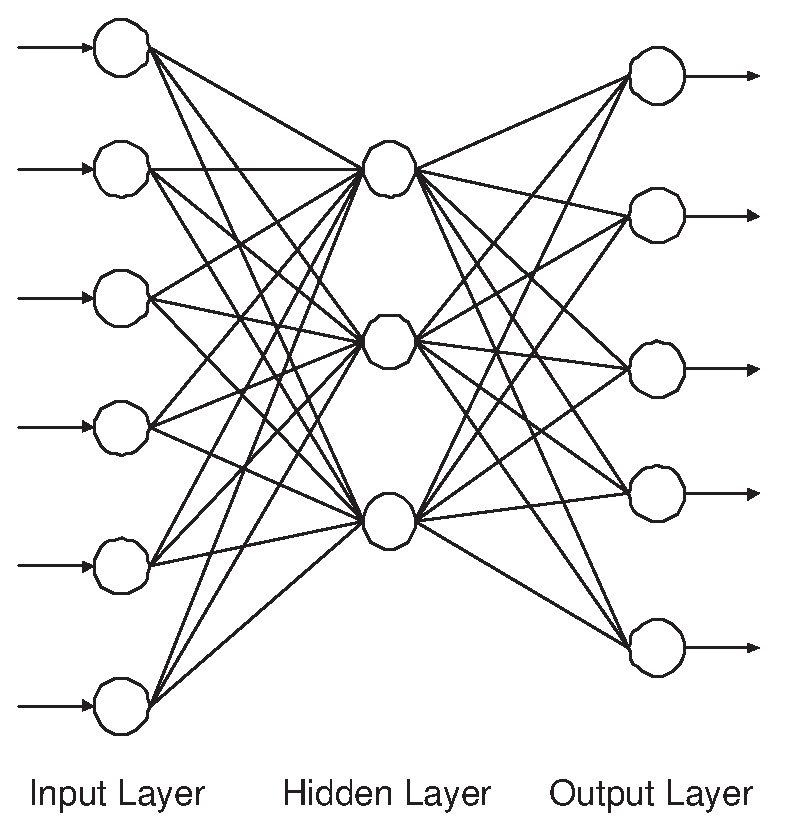
\includegraphics[width=2.5in]{NEURAL_NETWORK}
\caption{A Simple Neural Network Structure}
\label{fig_nn}
\end{figure}


Figure axis labels are often a source of confusion. Use words rather
than symbols. As an example, write the quantity "Magnetization," or
"Magnetization M," not just "M." Put units in parentheses. Do not
label axes only with units.

Large figures and tables may span both columns. Place figure
captions below the figures; place table titles above the tables. If
your figure has two parts, include the labels "(a)" and "(b)" as
part of the artwork. Please verify that the figures and tables you
mention in the text actually exist.


% Note that IAENG typically puts floats only at the top, even when this
% results in a large percentage of a column being occupied by floats.


% An example of a double column floating figure using two subfigures.
% (The subfig.sty package must be loaded for this to work.)
% The subfigure \label commands are set within each subfloat command, the
% \label for the overall figure must come after \caption.
% \hfil must be used as a separator to get equal spacing.
% The subfigure.sty package works much the same way, except \subfigure is
% used instead of \subfloat.
%
%\begin{figure*}[!t]
%\centerline{\subfloat[Case I]\includegraphics[width=2.5in]{subfigcase1}%
%\label{fig_first_case}}
%\hfil
%\subfloat[Case II]{\includegraphics[width=2.5in]{subfigcase2}%
%\label{fig_second_case}}}
%\caption{Simulation results}
%\label{fig_sim}
%\end{figure*}
%
% Note that often IAENG papers with subfigures do not employ subfigure
% captions (using the optional argument to \subfloat), but instead will
% reference/describe all of them (a), (b), etc., within the main caption.


% An example of a floating table. Note that, for IAENG style tables, the
% \caption command should come BEFORE the table. Table text will default to
% \footnotesize as IAENG normally uses this smaller font for tables.
% The \label must come after \caption as always.
%
%\begin{table}[!t]
%% increase table row spacing, adjust to taste
%\renewcommand{\arraystretch}{1.3}
% if using array.sty, it might be a good idea to tweak the value of
% \extrarowheight as needed to properly center the text within the cells
%\caption{An Example of a Table}
%\label{table_example}
%\centering
%% Some packages, such as MDW tools, offer better commands for making tables
%% than the plain LaTeX2e tabular which is used here.
%\begin{tabular}{|c||c||c|}
%\hline
%One & Two & Five\\
%\hline
%Two & Four & Ten\\
%\hline
%\end{tabular}
%\end{table}

\begin{table}[!t]
\renewcommand{\arraystretch}{1.3}
\caption{An Example of a Table} \label{table_example}
\centering
\begin{tabular}{|c||c||c|}
\hline
One & Two & Five\\
\hline
Two & Four & Ten\\
\hline
\end{tabular}
\end{table}


% Note that IAENG does not put floats in the very first column - or typically
% anywhere on the first page for that matter. Also, in-text middle ("here")
% positioning is not used. Most IAENG journals use top floats exclusively.
% Note that, LaTeX2e, unlike IAENG journals, places footnotes above bottom
% floats. This can be corrected via the \fnbelowfloat command of the
% stfloats package.



\section{Conclusion}
The conclusion goes here.

A conclusion section is not compulsory. Although a conclusion may
review the main points of the paper, do not replicate the abstract
as the conclusion. A conclusion might elaborate on the importance of
the work or suggest applications and extensions
\cite{IAENGhowto:kopka, IJCS, EL, IJAM, WCECS, WCE, IMECS}.




% if have a single appendix:
%\appendix[Proof of the Zonklar Equations]
% or
%\appendix  % for no appendix heading
% do not use \section anymore after \appendix, only \section*
% is possibly needed

% use appendices with more than one appendix
% then use \section to start each appendix
% you must declare a \section before using any
% \subsection or using \label (\appendices by itself
% starts a section numbered zero.)
%


\appendices
\section{Proof of the First Zonklar Equation}
Appendix one text goes here.

% you can choose not to have a title for an appendix
% if you want by leaving the argument blank
\section{}
Appendix two text goes here.


% use section* for acknowledgement
\section*{Acknowledgment}


The authors would like to thank...

The preferred spelling of the word "acknowledgment" in American
English is without an "e" after the "g." Use the singular heading
even if you have many acknowledgments. Avoid expressions such as
"One of us (S.B.A.) would like to thank ... ." Instead, write "F. A.
Author thanks ... ." Sponsor and financial support acknowledgments
are placed in the unnumbered footnote on the first page, not here.


% Can use something like this to put references on a page
% by themselves when using endfloat and the captionsoff option.
\ifCLASSOPTIONcaptionsoff
  \newpage
\fi



% trigger a \newpage just before the given reference
% number - used to balance the columns on the last page
% adjust value as needed - may need to be readjusted if
% the document is modified later
%\IAENGtriggeratref{8}
% The "triggered" command can be changed if desired:
%\IAENGtriggercmd{\enlargethispage{-5in}}

% references section

% can use a bibliography generated by BibTeX as a .bbl file
% BibTeX documentation can be easily obtained at:
% http://www.ctan.org/tex-archive/biblio/bibtex/contrib/doc/
% The IAENGtran BibTeX style support page is at:
% http://www.michaelshell.org/tex/IAENGtran/bibtex/
%\bibliographystyle{IAENGtran}
% argument is your BibTeX string definitions and bibliography database(s)
%\bibliography{IAENGabrv,../bib/paper}
%
% <OR> manually copy in the resultant .bbl file
% set second argument of \begin to the number of references
% (used to reserve space for the reference number labels box)
\begin{thebibliography}{1}

\bibitem{IAENGhowto:kopka}
H.~Kopka and P.~W. Daly, \emph{A Guide to \LaTeX}, 3rd~ed.\hskip 1em plus
  0.5em minus 0.4em\relax Harlow, England: Addison-Wesley, 1999.

\bibitem{IJCS}
N.~Meghanathan and G.~W. Skelton, ``Risk Notification Message
Dissemination Protocol for Energy Efficient Broadcast in Vehicular
Ad hoc Networks,'' {\it IAENG International Journal of Computer
Science}, vol. 37, no. 1, pp. 1-10, Jul. 2010.

\bibitem{EL}
E.~H. Miller, ``A note on reflector arrays (Periodical
style-Accepted for publication),'' {\it Engineering Letters}, to be
published.

\bibitem{IJAM}
J.~Wang, ``Fundamentals of erbium-doped fiber amplifiers arrays
(Periodical style-Submitted for publication),'' {\it IAENG
International Journal of Applied Mathematics}, submitted for
publication.

\bibitem{WCECS}
N.~Sohaee and C.~V. Rorst, ``Bounded Diameter Clustering Scheme For
Protein Interaction Networks,'' in {\it Lecture Notes in Engineering
and Computer Science: World Congress on Engineering and Computer
Science 2009}, pp. 1-7.

\bibitem{WCE}
J.~M. Merigo, ``Using the Probabilistic Weight Average in Decision
Making with Distsance Measures,'' in {\it Lecture Notes in
Engineering and Computer Science: World Congress on Engineering
2010}, pp. 1-4.

\bibitem{IMECS}
T.~Gonsalves and K.~Itoh, ``Multi-Objective Optimization for
Software Development Projects,'' in {\it Lecture Notes in
Engineering and Computer Science: International Multiconference of
Engineers and Computer Scientist 2010}, pp. 1-6.


\end{thebibliography}


\end{document}
